\documentclass{standalone}
\usepackage{tikz}
\usetikzlibrary{patterns, positioning}

\begin{document}
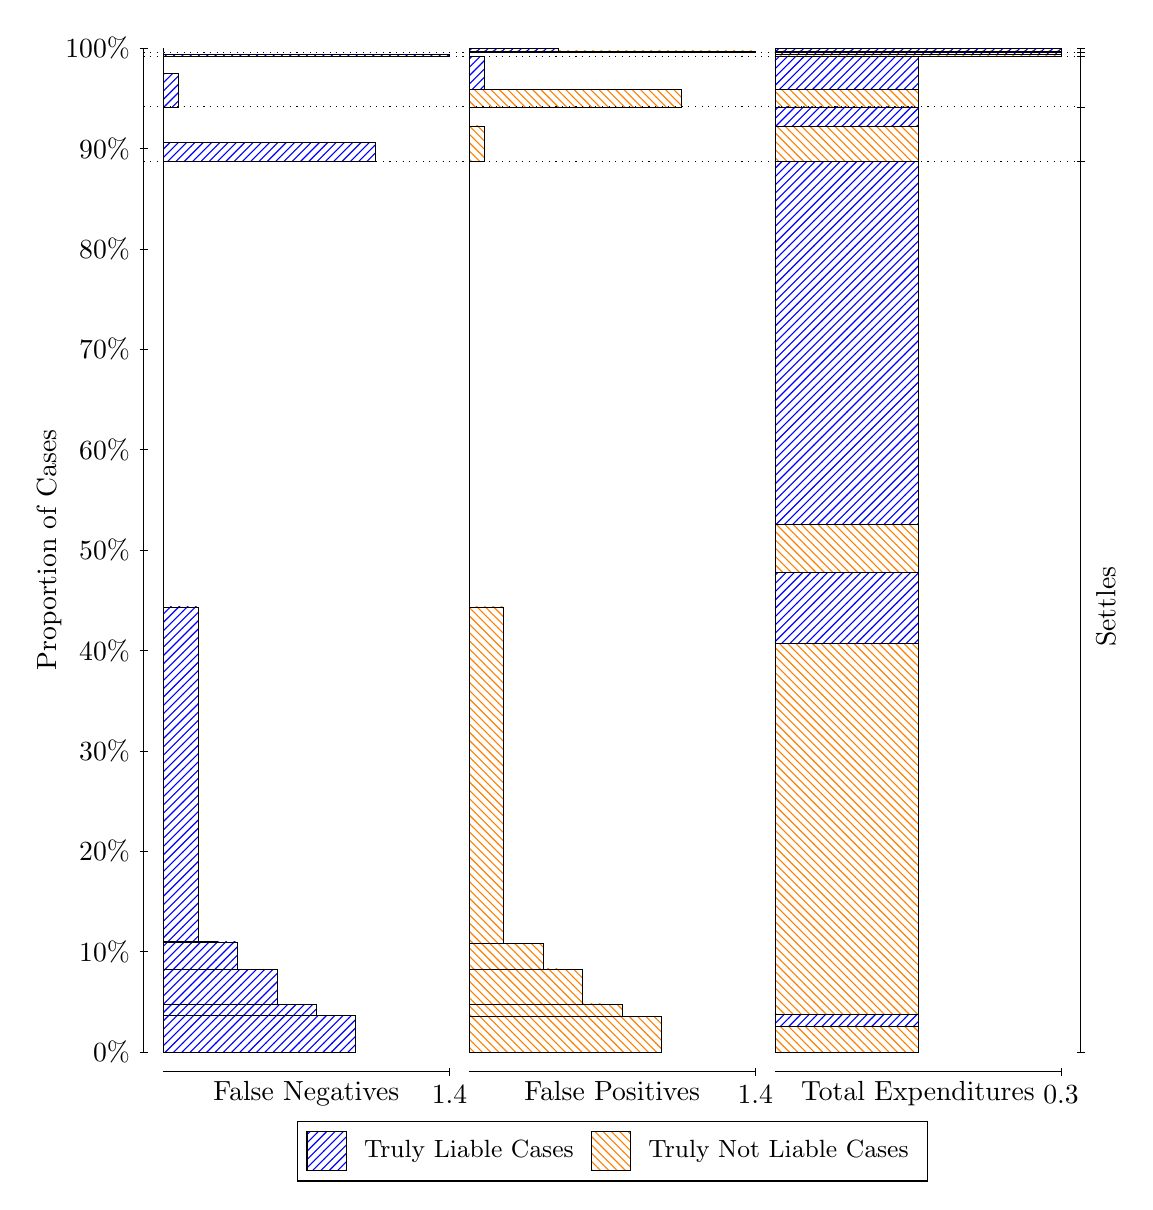
\begin{tikzpicture}
\draw[black, very thin] (1.5,1.75) -- (1.5,14.5);
\node[rotate=90, anchor=center] at (0.3, 8.125) {Proportion of Cases};
\draw[black, very thin] (1.45,1.75) -- (1.55,1.75);
\node[anchor=east] at (1.45, 1.75) {0\%};
\draw[black, very thin] (1.45,3.025) -- (1.55,3.025);
\node[anchor=east] at (1.45, 3.025) {10\%};
\draw[black, very thin] (1.45,4.3) -- (1.55,4.3);
\node[anchor=east] at (1.45, 4.3) {20\%};
\draw[black, very thin] (1.45,5.575) -- (1.55,5.575);
\node[anchor=east] at (1.45, 5.575) {30\%};
\draw[black, very thin] (1.45,6.85) -- (1.55,6.85);
\node[anchor=east] at (1.45, 6.85) {40\%};
\draw[black, very thin] (1.45,8.125) -- (1.55,8.125);
\node[anchor=east] at (1.45, 8.125) {50\%};
\draw[black, very thin] (1.45,9.4) -- (1.55,9.4);
\node[anchor=east] at (1.45, 9.4) {60\%};
\draw[black, very thin] (1.45,10.675) -- (1.55,10.675);
\node[anchor=east] at (1.45, 10.675) {70\%};
\draw[black, very thin] (1.45,11.95) -- (1.55,11.95);
\node[anchor=east] at (1.45, 11.95) {80\%};
\draw[black, very thin] (1.45,13.225) -- (1.55,13.225);
\node[anchor=east] at (1.45, 13.225) {90\%};
\draw[black, very thin] (1.45,14.5) -- (1.55,14.5);
\node[anchor=east] at (1.45, 14.5) {100\%};

\draw[black, very thin] (13.4,1.75) -- (13.4,14.5);
\draw[black, very thin] (13.35,1.75) -- (13.45,1.75);
\node[anchor=west] at (13.35, 1.75) {};
\draw[black, very thin] (13.35,13.057) -- (13.45,13.057);
\node[anchor=west] at (13.35, 13.057) {};
\draw[black, very thin] (13.35,13.753) -- (13.45,13.753);
\node[anchor=west] at (13.35, 13.753) {};
\draw[black, very thin] (13.35,14.397) -- (13.45,14.397);
\node[anchor=west] at (13.35, 14.397) {};
\draw[black, very thin] (13.35,14.443) -- (13.45,14.443);
\node[anchor=west] at (13.35, 14.443) {};
\draw[black, very thin] (13.35,14.5) -- (13.45,14.5);
\node[anchor=west] at (13.35, 14.5) {};

\draw[black, very thin, pattern color=blue, pattern=north east lines] (1.75,1.75) rectangle (4.1931,2.2103);
\draw[black, very thin, pattern color=blue, pattern=north east lines] (1.75,2.2103) rectangle (3.9425,2.2113);
\draw[black, very thin, pattern color=blue, pattern=north east lines] (1.75,2.2113) rectangle (3.692,2.3551);
\draw[black, very thin, pattern color=blue, pattern=north east lines] (1.75,2.3551) rectangle (3.4414,2.3574);
\draw[black, very thin, pattern color=blue, pattern=north east lines] (1.75,2.3574) rectangle (3.1908,2.7993);
\draw[black, very thin, pattern color=blue, pattern=north east lines] (1.75,2.7993) rectangle (2.9402,2.8033);
\draw[black, very thin, pattern color=blue, pattern=north east lines] (1.75,2.8033) rectangle (2.6897,3.1494);
\draw[black, very thin, pattern color=blue, pattern=north east lines] (1.75,3.1494) rectangle (2.4391,3.1505);
\draw[black, very thin, pattern color=blue, pattern=north east lines] (1.75,3.1505) rectangle (2.1885,7.4036);
\draw[black, very thin, pattern color=orange, pattern=north west lines] (1.75,7.4036) rectangle (1.75,13.057);
\draw[black, very thin, pattern color=blue, pattern=north east lines] (1.75,13.057) rectangle (4.4437,13.3);
\draw[black, very thin, pattern color=orange, pattern=north west lines] (1.75,13.3) rectangle (1.75,13.753);
\draw[black, very thin, pattern color=blue, pattern=north east lines] (1.75,13.753) rectangle (1.9379,14.177);
\draw[black, very thin, pattern color=orange, pattern=north west lines] (1.75,14.177) rectangle (1.75,14.397);
\draw[black, very thin, pattern color=blue, pattern=north east lines] (1.75,14.397) rectangle (5.3833,14.417);
\draw[black, very thin, pattern color=orange, pattern=north west lines] (1.75,14.417) rectangle (1.75,14.443);
\draw[black, very thin, pattern color=orange, pattern=north west lines] (1.75,14.443) rectangle (1.75,14.465);
\draw[black, very thin, pattern color=blue, pattern=north east lines] (1.75,14.465) rectangle (1.75,14.5);
\draw[black, very thin, pattern color=orange, pattern=north west lines] (5.6333,1.75) rectangle (8.0764,2.2014);
\draw[black, very thin, pattern color=orange, pattern=north west lines] (5.6333,2.2014) rectangle (7.8259,2.2019);
\draw[black, very thin, pattern color=orange, pattern=north west lines] (5.6333,2.2019) rectangle (7.5753,2.3562);
\draw[black, very thin, pattern color=orange, pattern=north west lines] (5.6333,2.3562) rectangle (7.3247,2.3596);
\draw[black, very thin, pattern color=orange, pattern=north west lines] (5.6333,2.3596) rectangle (7.0741,2.8016);
\draw[black, very thin, pattern color=orange, pattern=north west lines] (5.6333,2.8016) rectangle (6.8236,2.8029);
\draw[black, very thin, pattern color=orange, pattern=north west lines] (5.6333,2.8029) rectangle (6.8236,2.8052);
\draw[black, very thin, pattern color=orange, pattern=north west lines] (5.6333,2.8052) rectangle (6.573,3.1281);
\draw[black, very thin, pattern color=orange, pattern=north west lines] (5.6333,3.1281) rectangle (6.3224,3.1302);
\draw[black, very thin, pattern color=orange, pattern=north west lines] (5.6333,3.1302) rectangle (6.0718,7.4034);
\draw[black, very thin, pattern color=blue, pattern=north east lines] (5.6333,7.4034) rectangle (5.6333,13.057);
\draw[black, very thin, pattern color=orange, pattern=north west lines] (5.6333,13.057) rectangle (5.8213,13.51);
\draw[black, very thin, pattern color=blue, pattern=north east lines] (5.6333,13.51) rectangle (5.6333,13.753);
\draw[black, very thin, pattern color=orange, pattern=north west lines] (5.6333,13.753) rectangle (8.327,13.974);
\draw[black, very thin, pattern color=blue, pattern=north east lines] (5.6333,13.974) rectangle (5.8213,14.397);
\draw[black, very thin, pattern color=orange, pattern=north west lines] (5.6333,14.397) rectangle (5.6333,14.423);
\draw[black, very thin, pattern color=blue, pattern=north east lines] (5.6333,14.423) rectangle (5.6333,14.443);
\draw[black, very thin, pattern color=orange, pattern=north west lines] (5.6333,14.443) rectangle (9.2667,14.465);
\draw[black, very thin, pattern color=blue, pattern=north east lines] (5.6333,14.465) rectangle (6.7609,14.5);
\draw[black, very thin, pattern color=orange, pattern=north west lines] (9.5167,1.75) rectangle (11.333,2.0786);
\draw[black, very thin, pattern color=blue, pattern=north east lines] (9.5167,2.0786) rectangle (11.333,2.2256);
\draw[black, very thin, pattern color=orange, pattern=north west lines] (9.5167,2.2256) rectangle (11.333,6.9409);
\draw[black, very thin, pattern color=blue, pattern=north east lines] (9.5167,6.9409) rectangle (11.333,7.8432);
\draw[black, very thin, pattern color=orange, pattern=north west lines] (9.5167,7.8432) rectangle (11.333,8.4527);
\draw[black, very thin, pattern color=blue, pattern=north east lines] (9.5167,8.4527) rectangle (11.333,13.057);
\draw[black, very thin, pattern color=orange, pattern=north west lines] (9.5167,13.057) rectangle (11.333,13.51);
\draw[black, very thin, pattern color=blue, pattern=north east lines] (9.5167,13.51) rectangle (11.333,13.753);
\draw[black, very thin, pattern color=orange, pattern=north west lines] (9.5167,13.753) rectangle (11.333,13.974);
\draw[black, very thin, pattern color=blue, pattern=north east lines] (9.5167,13.974) rectangle (11.333,14.397);
\draw[black, very thin, pattern color=orange, pattern=north west lines] (9.5167,14.397) rectangle (13.15,14.423);
\draw[black, very thin, pattern color=blue, pattern=north east lines] (9.5167,14.423) rectangle (13.15,14.443);
\draw[black, very thin, pattern color=orange, pattern=north west lines] (9.5167,14.443) rectangle (13.15,14.465);
\draw[black, very thin, pattern color=blue, pattern=north east lines] (9.5167,14.465) rectangle (13.15,14.5);
\draw[black, dotted] (1.5,13.057) -- (13.4,13.057);
\draw[black, dotted] (1.5,13.753) -- (13.4,13.753);
\draw[black, dotted] (1.5,14.397) -- (13.4,14.397);
\draw[black, dotted] (1.5,14.443) -- (13.4,14.443);
\draw[black, very thin] (1.75,1.5) -- (5.3833,1.5);
\node[anchor=north] at (3.5667, 1.5) {False Negatives};
\draw[black, very thin] (5.3833,1.45) -- (5.3833,1.55);
\node[anchor=north] at (5.3833, 1.45) {1.4};

\draw[black, very thin] (5.6333,1.5) -- (9.2667,1.5);
\node[anchor=north] at (7.45, 1.5) {False Positives};
\draw[black, very thin] (9.2667,1.45) -- (9.2667,1.55);
\node[anchor=north] at (9.2667, 1.45) {1.4};

\draw[black, very thin] (9.5167,1.5) -- (13.15,1.5);
\node[anchor=north] at (11.333, 1.5) {Total Expenditures};
\draw[black, very thin] (13.15,1.45) -- (13.15,1.55);
\node[anchor=north] at (13.15, 1.45) {0.3};

\node[black, centered, rotate=90] at (13.72, 7.4035) {Settles};





\draw (7.449999999999999,1.5) node[draw=none] (baseCoordinate) {};
\begin{scope}[align=center]
        \matrix[scale=0.5, draw=black, below=0.5cm of baseCoordinate, nodes={draw}, column sep=0.1cm]{
            \node[rectangle, draw, minimum width=0.5cm, minimum height=0.5cm, pattern=north east lines, pattern color=blue] {}; &
            \node[draw=none, font=\small] (B) {Truly Liable Cases}; &
            \node[rectangle, draw, minimum width=0.5cm, minimum height=0.5cm, pattern=north west lines, pattern color=orange] {}; &
            \node[draw=none, font=\small] (B) {Truly Not Liable Cases}; \\
            };
\end{scope}

\end{tikzpicture}
\end{document}